%\documentclass[mathserif]{beamer}              %use this for creating the presentation
\documentclass[handout,mathserif]{beamer}       %use this for creating the handout (i.e. no animation)
\usepackage{amsmath}
\usepackage{amssymb}
\usepackage{amsthm}
\usepackage{graphicx}
%\usepackage{subfig}

\usecolortheme{orchid}

\newcommand{\alignbox}[1]
    {\begin{equation*} \boxed{ \begin{aligned} #1
    \end{aligned} } \end{equation*}}
\newcommand{\gatherbox}[1]
    {\begin{equation*} \boxed{ \begin{gathered} #1
    \end{gathered} } \end{equation*}}
\newcommand{\ejw}{e^{j\omega}}
\newcommand{\paused}{\vspace*{-\baselineskip}\pause}     %use this if \pause puts too much space before the next line

%\input{../commands}
%\setkeys{Gin}{draft=true}

\setlength{\parskip}{10pt plus 1pt minus 1pt}

\title{ME 233 -- Advanced Control II\\
    Lecture 14 \\
    Disturbance Observers}
\author{Richard Conway}
\institute{UC Berkeley}


\begin{document}

\maketitle

\begin{frame}
    \frametitle{Outline}
    \tableofcontents
\end{frame}

\section{Motivation}
\begin{frame}
    \frametitle{Outline}
    \tableofcontents[currentsection]
\end{frame}

\begin{frame}
    \frametitle{Motivation}

    Consider the following plant structure
    \begin{figure}
        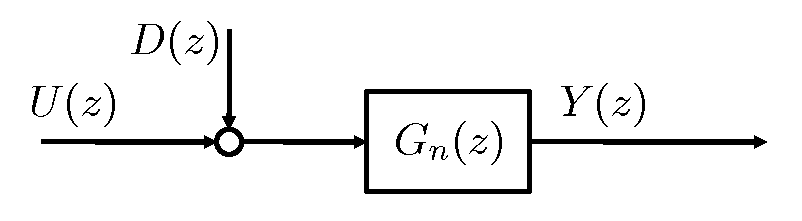
\includegraphics[width=0.5\textwidth]{Disturbance_Observer_motiv1}\\
    \end{figure}

    The signals are:

    \begin{center}
    \begin{tabular}{l @{ : } l}
        $U(z)$ & control input \\
        $D(z)$ & disturbance \\
        $Y(z)$ & output
    \end{tabular}
    \end{center}
    \pause

    The goal is to cancel the effect of $D(z)$ on $Y(z)$
\end{frame}

\begin{frame}
    \frametitle{Motivation}
    \begin{itemize}
    \item
    Let the plant be given by the transfer function $G_n(z)$, which is \underline{minimum phase} (i.e.\ its poles and zeros are strictly inside the unit disk in the complex plane)
    \pause

    \item
    Use an inverse plant to reconstruct $U(z) + D(z)$:
    \begin{figure}
        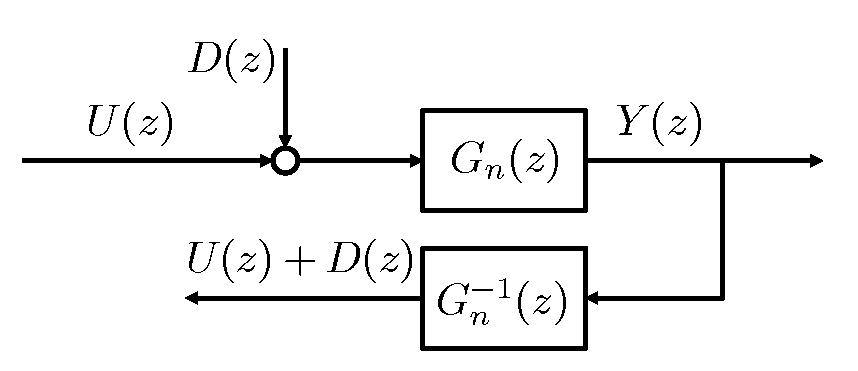
\includegraphics[width=0.5\textwidth]{Disturbance_Observer_motiv2}\\
    \end{figure}
    \pause

    \item
    Subtract $U(z)$ to reconstruct $D(z)$:
    \begin{figure}
        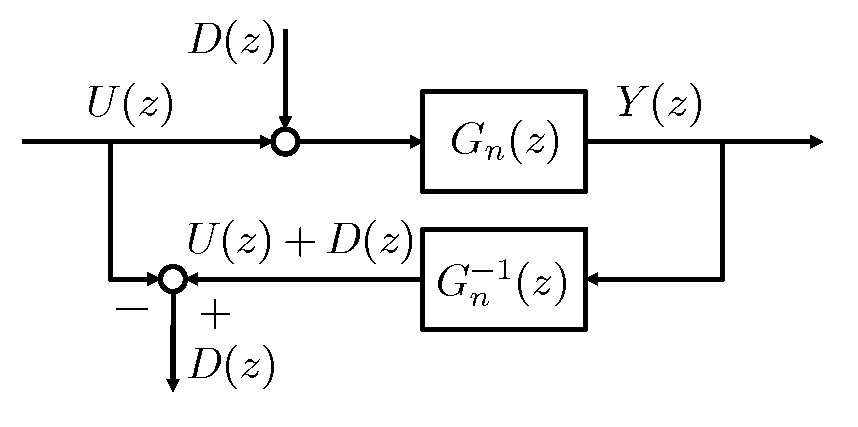
\includegraphics[width=0.5\textwidth]{Disturbance_Observer_motiv3}\\
    \end{figure}

    \end{itemize}
\end{frame}

\begin{frame}
    \frametitle{Motivation}
    \begin{itemize}
    \item
    Ideally, we would subtract the reconstructed value of $D(z)$ from $U(z)$
    \begin{figure}
        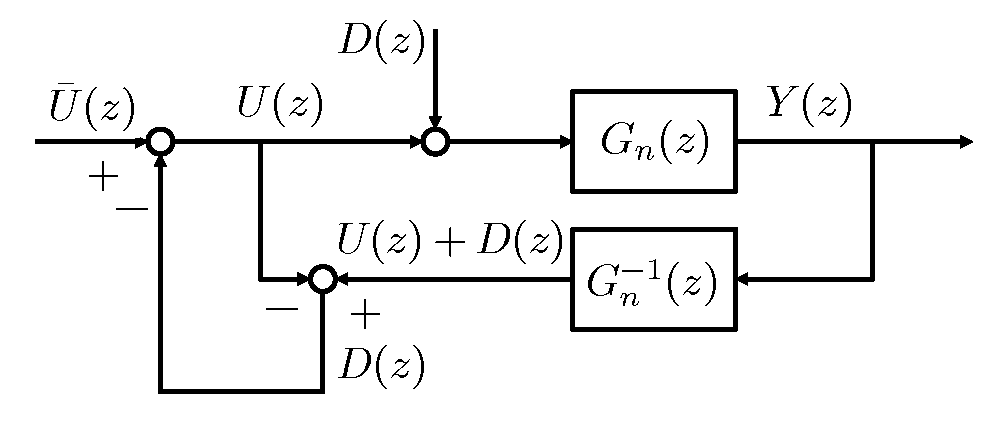
\includegraphics[width=0.7\textwidth]{Disturbance_Observer_motiv4}\\
    \end{figure}
    \pause

    \item
    This would yield the closed-loop dynamics $Y(z) = G_n(z) \bar{U}(z)$
    \end{itemize}
    \pause


    This controller structure would reconstruct $D(z)$ then subtract it from $U(z)$ so that the effect of the disturbance is \underline{exactly canceled}
    \pause

    $\Rightarrow$ This would be useful as an inner loop of a larger control scheme, \underline{BUT...}

\end{frame}

\begin{frame}
    \frametitle{Motivation---Problems}
    \begin{figure}
        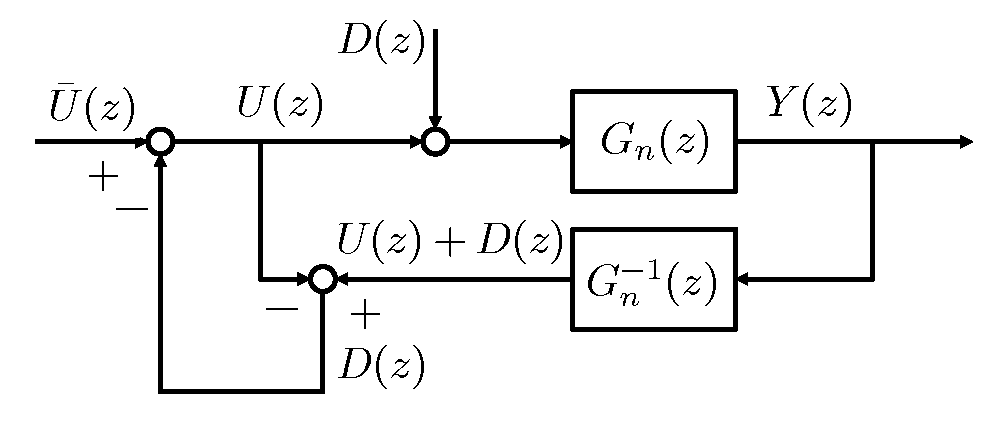
\includegraphics[width=0.5\textwidth]{Disturbance_Observer_motiv4}\\
    \end{figure}

    The control structure has some problems that should be resolved in order for it to be useful:

    \begin{itemize}
    \item
    Since $G_n^{-1}(z)$ is typically not proper, it is not realizable
    \pause

    $\Rightarrow$ We cannot reconstruct $D(z)$
    \pause

    \item
    The system being controlled might not be exactly as given by the model $G_n(z)$
    \pause

    \item
    Sensor noise will corrupt the reconstructed value of $D(z)$
    \pause
    
    \item
    The block diagram above is not well-posed and, in particular, $U(z)$ is not a realizable function of $Y(z)$.

    \end{itemize}
\end{frame}



\section{Disturbance observer}
\begin{frame}
    \frametitle{Outline}
    \tableofcontents[currentsection]
\end{frame}

\begin{frame}
    \frametitle{Disturbance Observer}

    The following control structure is referred to as a disturbance observer:
    \begin{figure}
        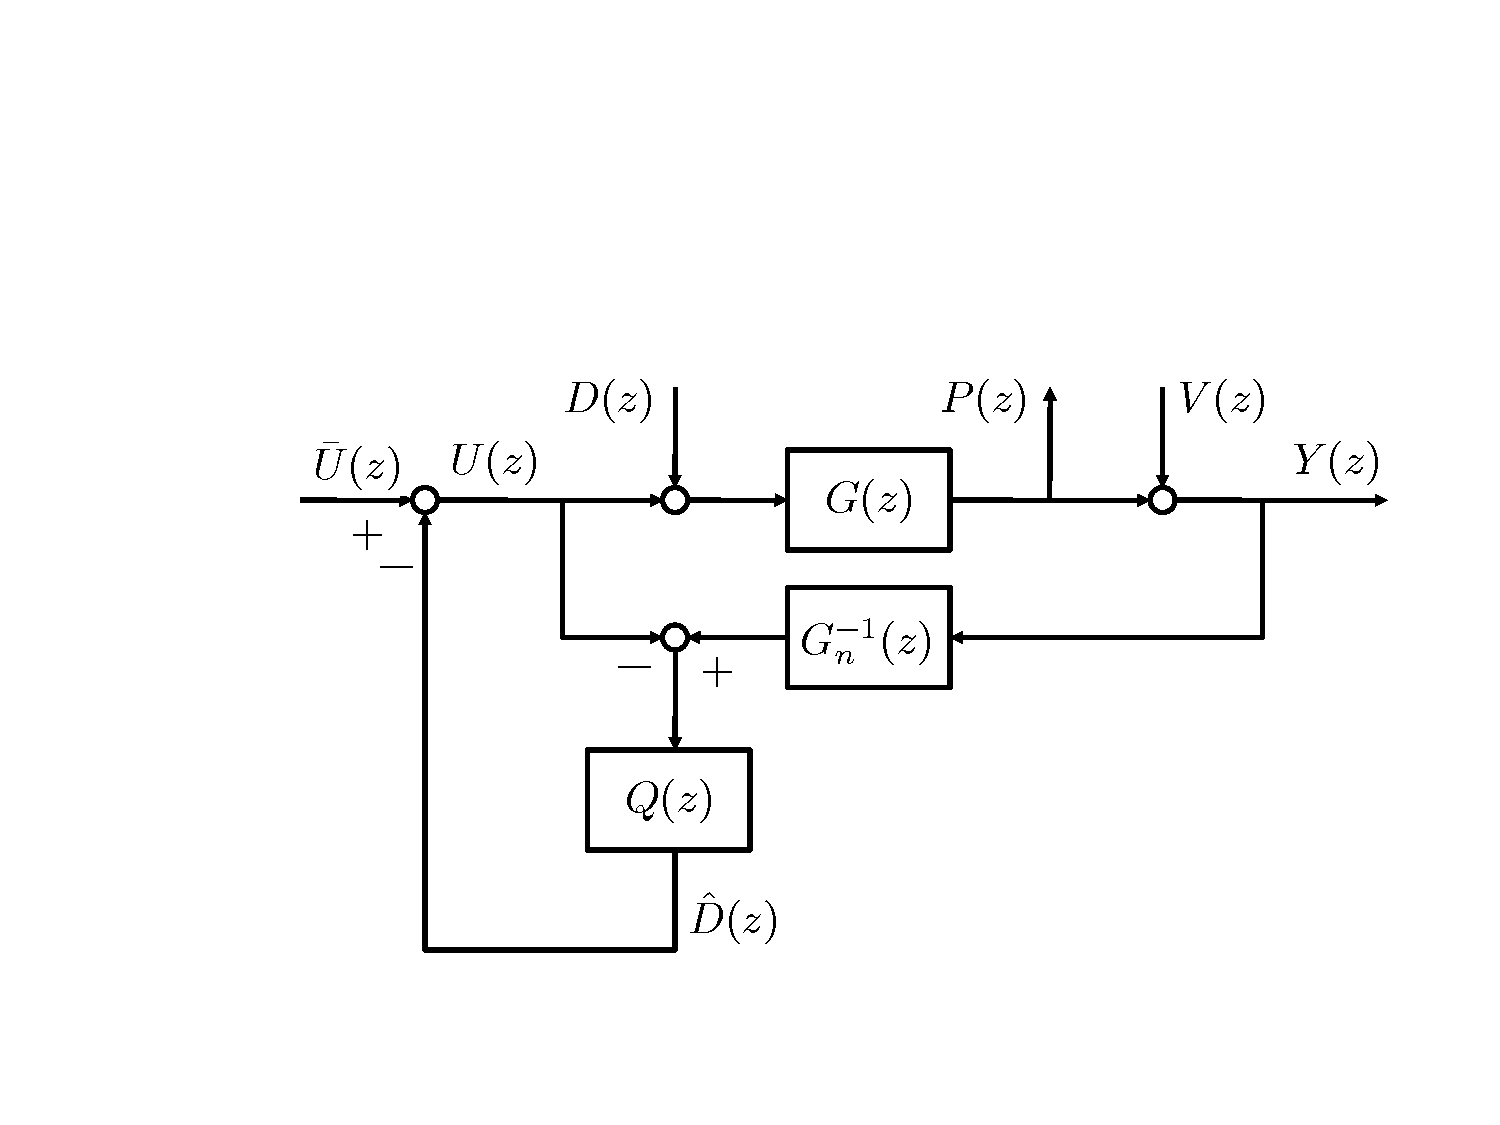
\includegraphics[width=0.7\textwidth]{Disturbance_Observer_DO}\\
    \end{figure}

    The signals are:

    \begin{center}
    \begin{tabular}{l @{ : } lll @{ : } l}
        $U(z)$ & control input && $V(z)$ & measurement noise \\
        $D(z)$ & disturbance && $\hat{D}(z)$ & estimate of $D(z)$ \\
        $Y(z)$ & measured output && $P(z)$ & performance output
    \end{tabular}
    \end{center}
\end{frame}

\begin{frame}
    \frametitle{Disturbance Observer}

    \begin{figure}
        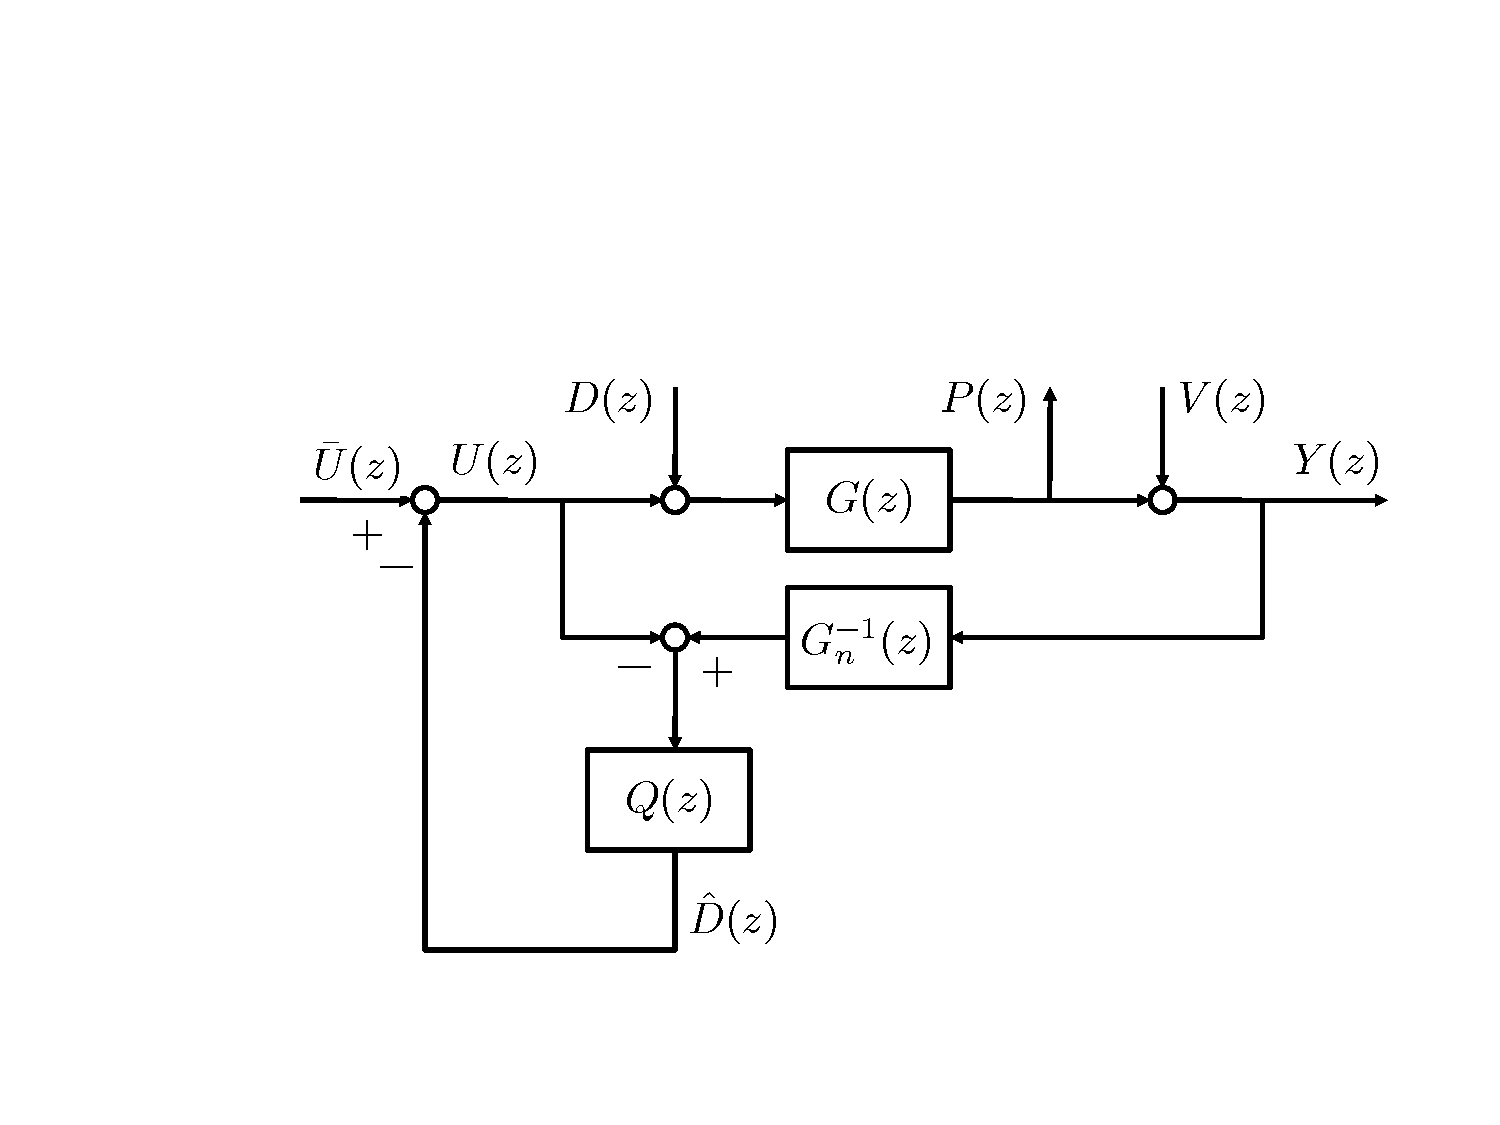
\includegraphics[width=0.7\textwidth]{Disturbance_Observer_DO}\\
    \end{figure}

    \begin{itemize}
    \item
    The one difference in the control architecture (compared to the motivation) is the presence of $Q(z)$

    \item
    $Q(z)$ is used to make the dynamics from $U(z)$ and $Y(z)$ to $\hat{D}(z)$ realizable
    \end{itemize}
\end{frame}

\begin{frame}
    \frametitle{Disturbance Observer---Comparison to Motivation}

    \begin{figure}
        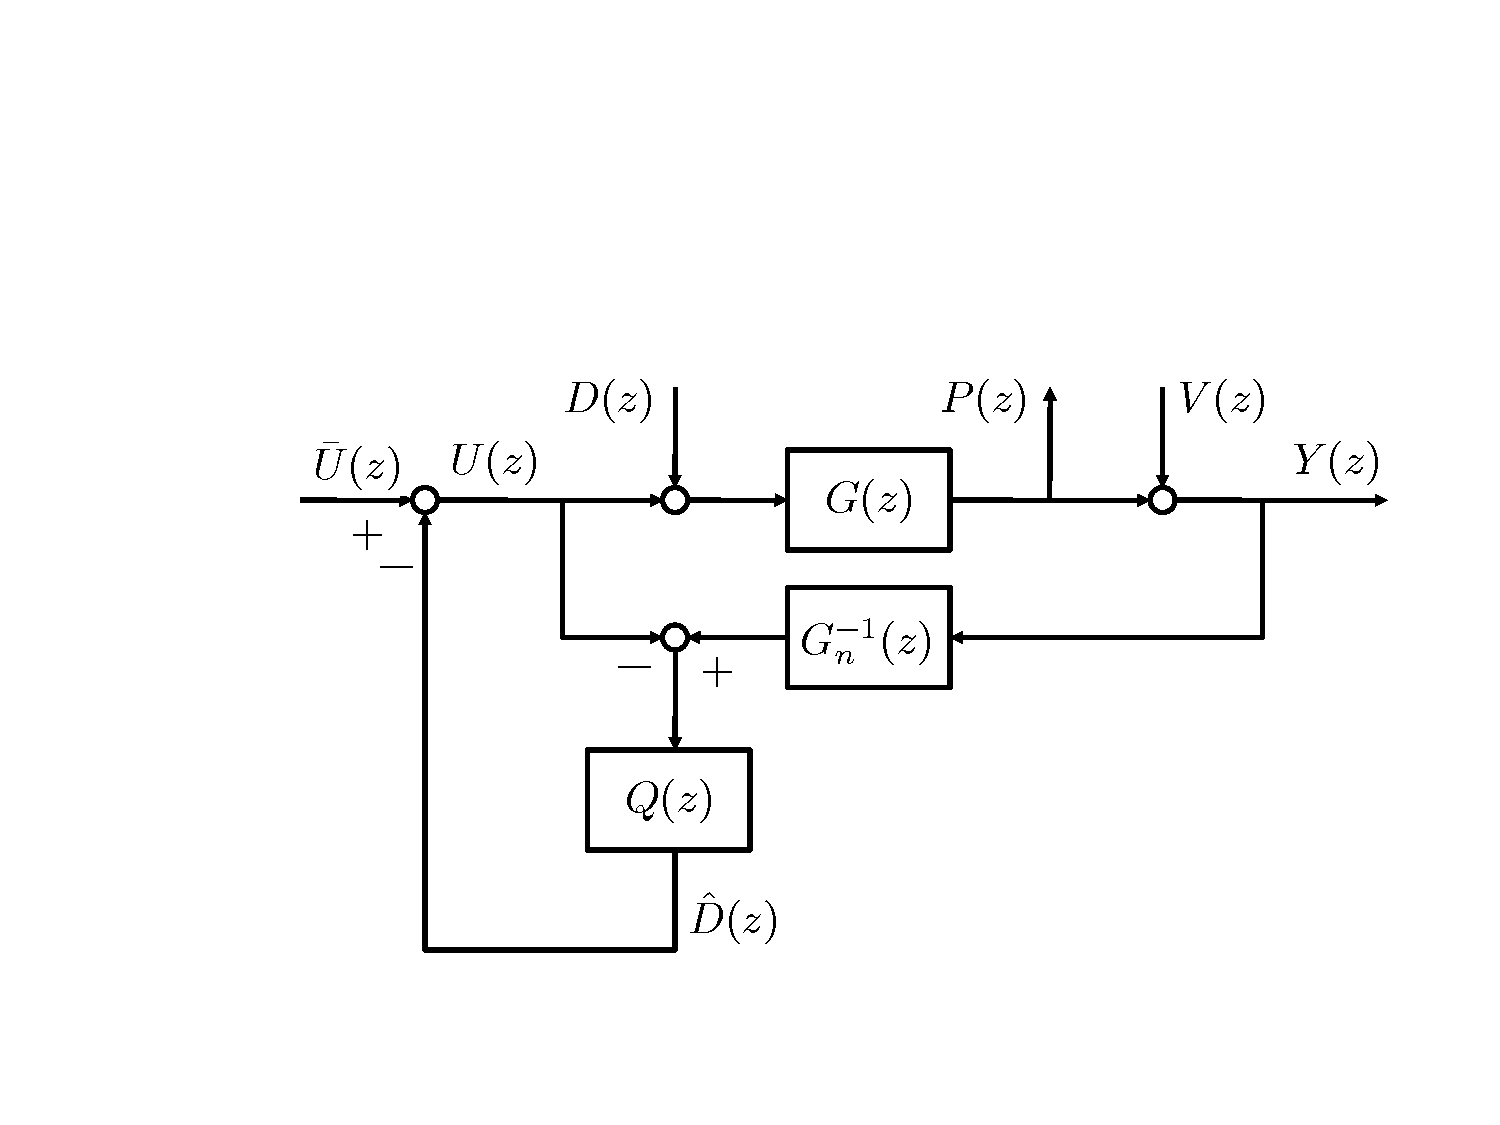
\includegraphics[width=0.7\textwidth]{Disturbance_Observer_DO}\\
    \end{figure}

    The structure in the Motivation section corresponds to
    \begin{itemize}
    \item
    $G(z) = G_n(z)$ (the plant is exactly as modeled)
    \pause

    \item
    $V(z) = 0$ (there is no sensor noise)
    \pause

    \item
    $Q(z) = 1$ (it is possible to realize $G_n^{-1}(z)$ )

    \end{itemize}
\end{frame}



\section{Derivation of closed-loop dynamics}
\begin{frame}
    \frametitle{Outline}
    \tableofcontents[currentsection]
\end{frame}

\begin{frame}
    \frametitle{Derivation of closed-loop dynamics}

    \begin{figure}
        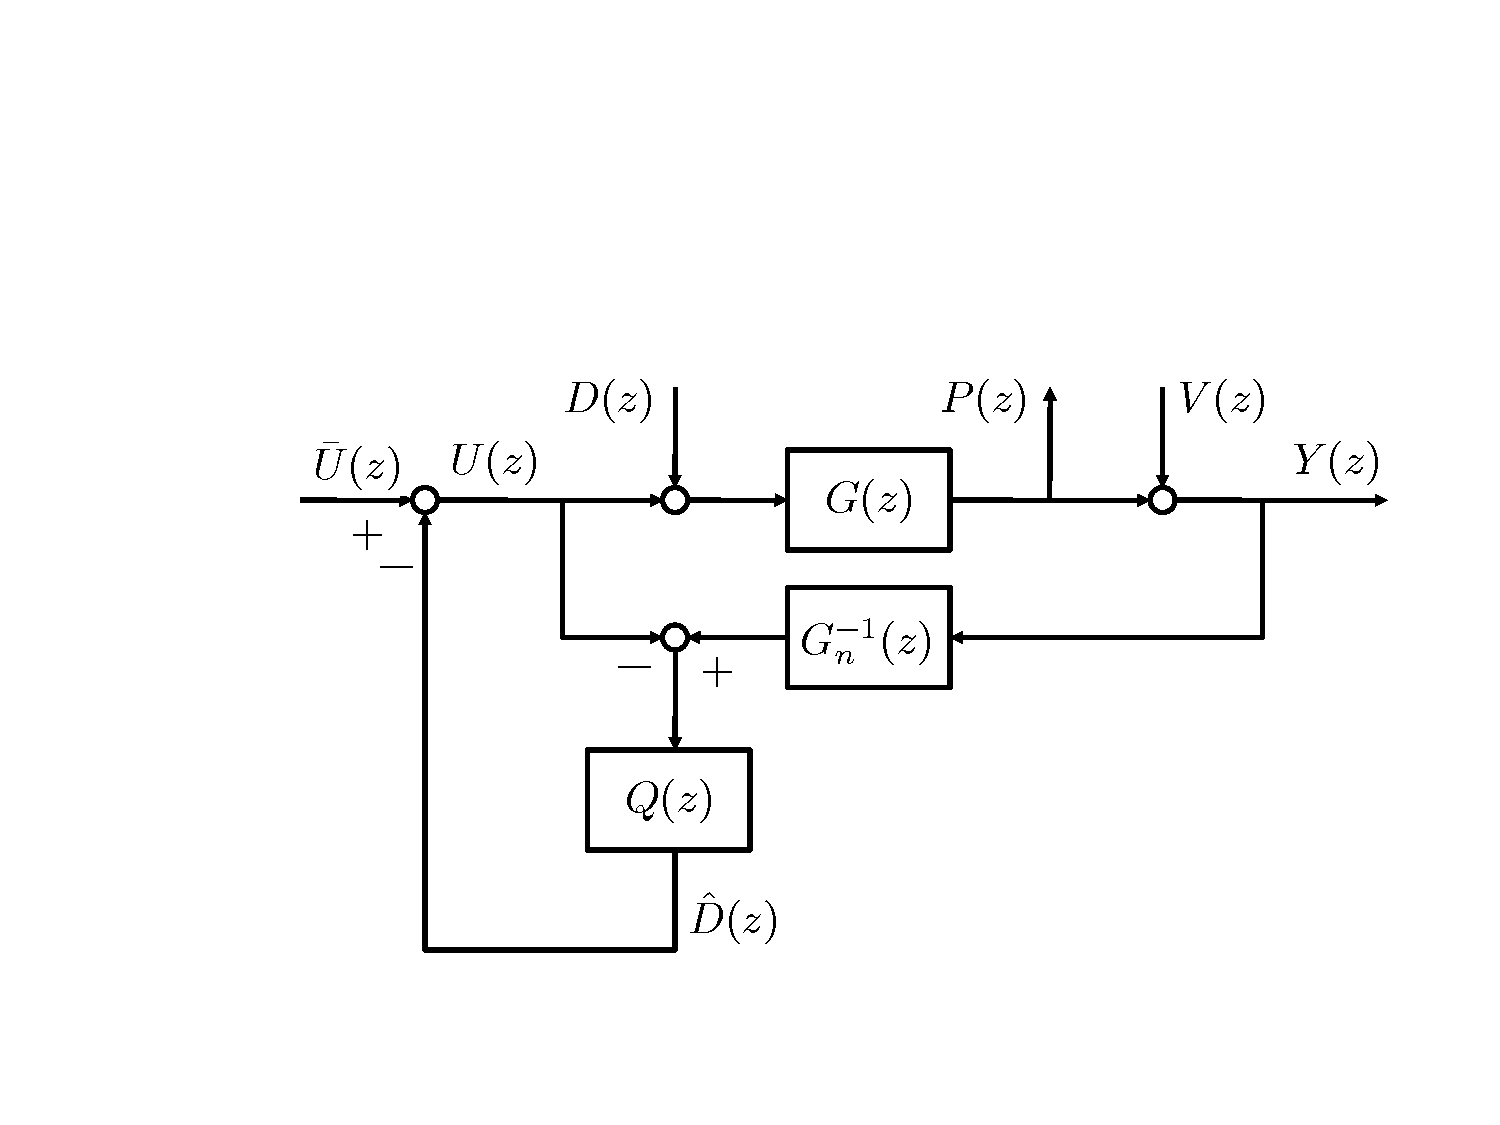
\includegraphics[width=0.5\textwidth]{Disturbance_Observer_DO}\\
    \end{figure}

    We will omit the dependency on $z$ to shorten notation
    \pause

    Plant dynamics: $Y = G(U+D) + V$
    \pause

    Now find the disturbance estimate $\hat{D}$ in terms of $U$, $D$, and $V$:
    \pause
    \begin{gather*}
        \hat{D} = Q (G_n^{-1} Y - U) \\
        \Rightarrow \quad \hat{D} = Q [ G_n^{-1} G (U+D) + G_n^{-1} V - U ] \\
        \Rightarrow \quad \hat{D} = Q ( G_n^{-1} G - 1) U + Q G_n^{-1} GD + QG_n^{-1} V
    \end{gather*}
\end{frame}

\begin{frame}
    \frametitle{Derivation of closed-loop dynamics}

    \begin{figure}
        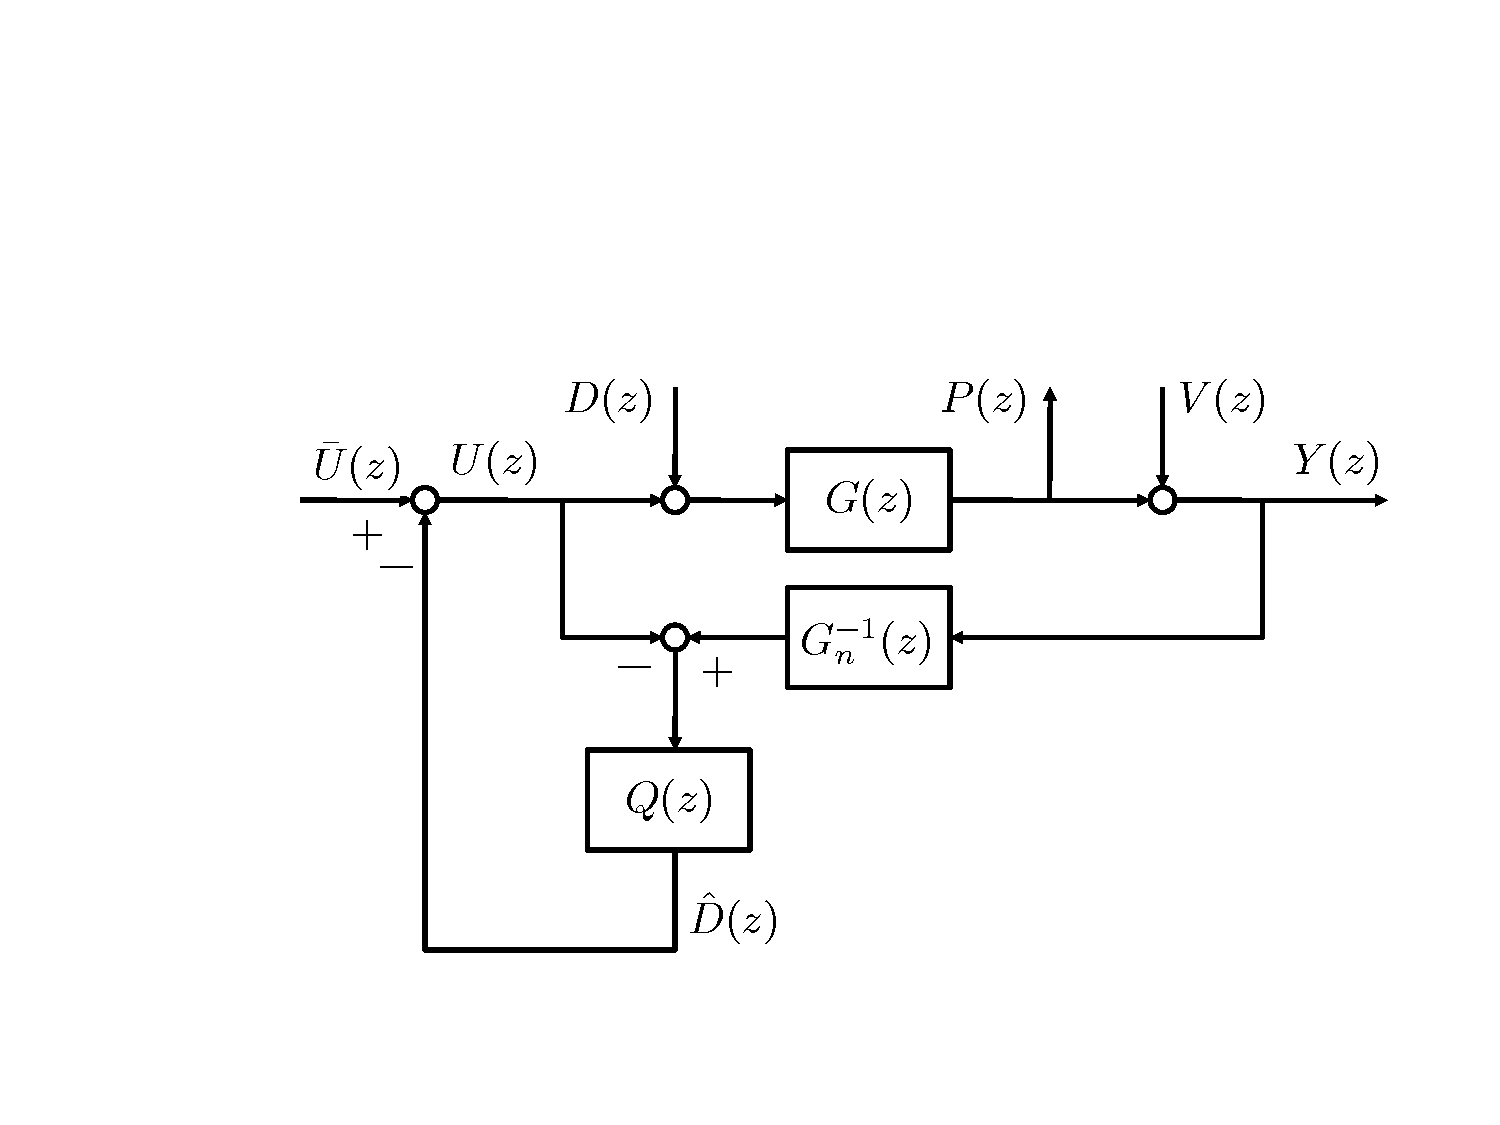
\includegraphics[width=0.5\textwidth]{Disturbance_Observer_DO}\\
    \end{figure}

    Solve for $U$ in terms of $D$, $\bar{U}$, and $V$:
    \begin{gather*}
        U = \bar{U} - \hat{D} \\
        \Rightarrow \quad U = \bar{U} - Q ( G_n^{-1} G - 1) U - Q G_n^{-1} GD - QG_n^{-1} V \\
        \Rightarrow \quad [1 + Q ( G_n^{-1} G - 1)] U = \bar{U} - Q G_n^{-1} GD - QG_n^{-1} V
    \end{gather*}
    \pause
    Now that we have $U$ in terms of $D$, $\bar{U}$, and $V$, we can solve for $P$ in terms of $D$, $\bar{U}$, and $V$
\end{frame}

\begin{frame}
    \frametitle{Derivation of closed-loop dynamics}

    \begin{figure}
        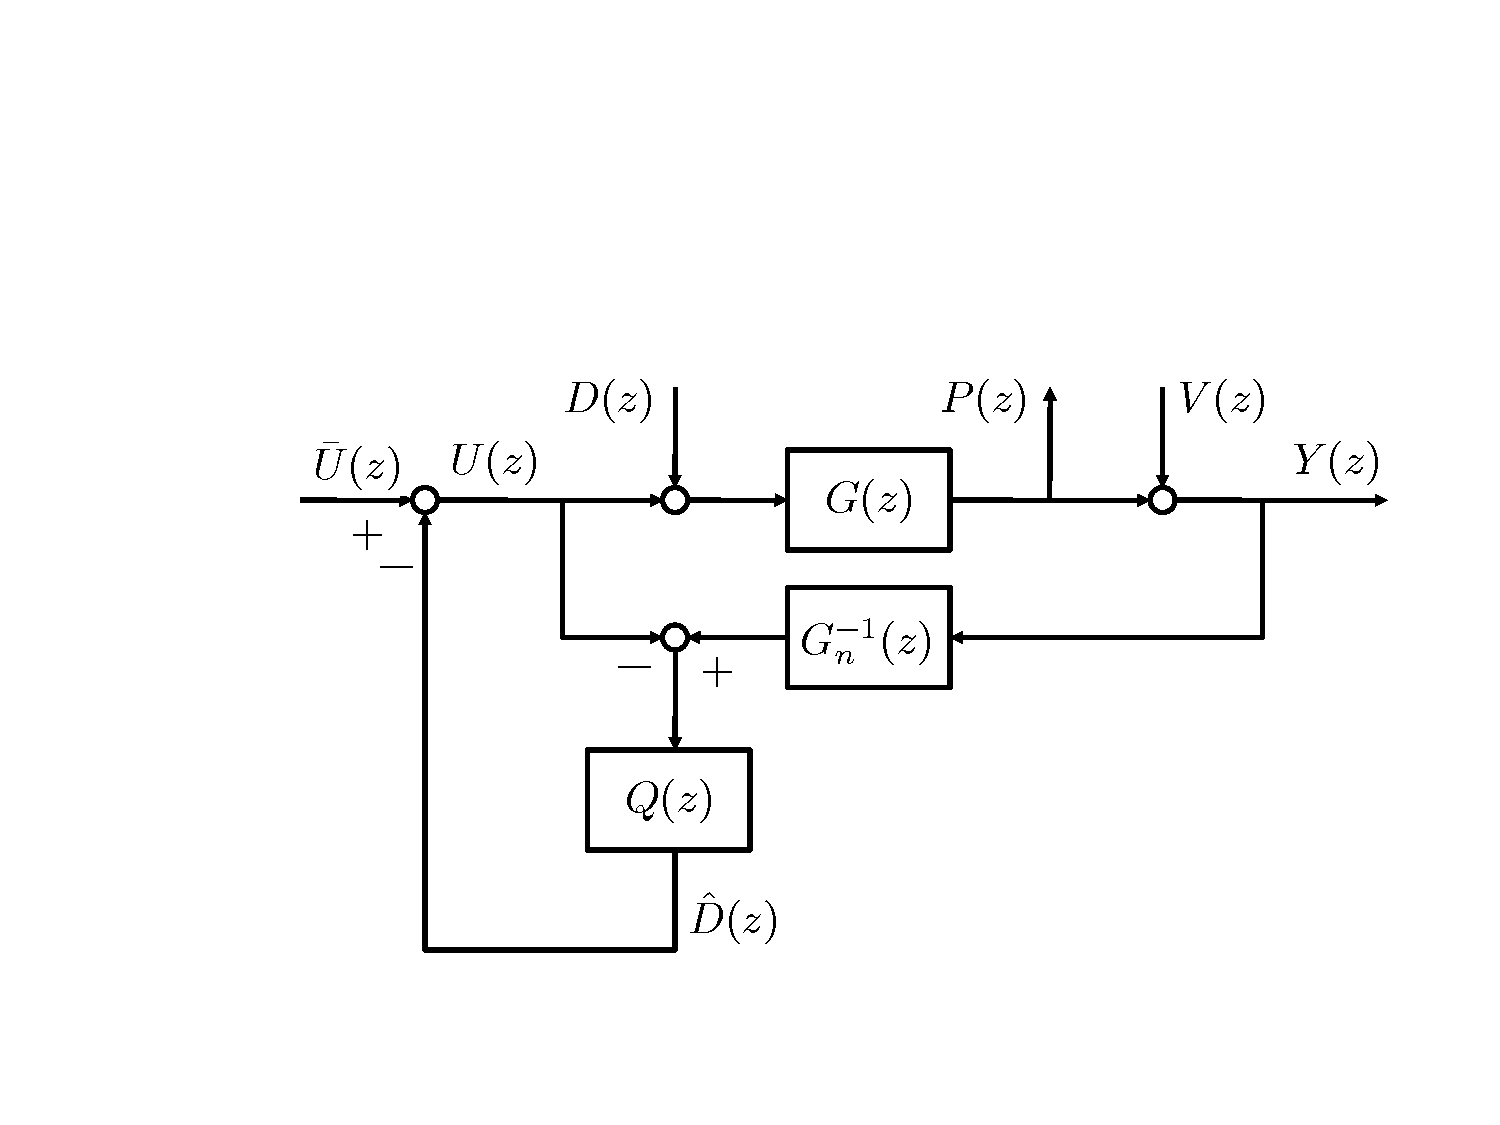
\includegraphics[width=0.3\textwidth]{Disturbance_Observer_DO}\\
    \end{figure}

    Solve for $P$ in terms of $D$, $\bar{U}$, and $V$:
    \begin{gather*}
        P = GD + GU \\
        \Rightarrow \quad P = GD + \frac{G}{1 + Q ( G_n^{-1} G - 1)} 
            [ \bar{U} - Q G_n^{-1} GD - QG_n^{-1} V ]
    \end{gather*}
    \pause
    \alignbox{
        P & = \frac{G (1-Q)}{1 + Q ( G_n^{-1} G - 1)} D + \frac{G}{1 + Q ( G_n^{-1} G - 1)} \bar{U} \\
        & \quad - \frac{GQ G_n^{-1}}{1 + Q ( G_n^{-1} G - 1)} V
    }
\end{frame}

\begin{frame}
    \frametitle{Derivation of closed-loop dynamics}

    \begin{align*}
        P & = \frac{G (1-Q)}{1 + Q ( G_n^{-1} G - 1)} D + \frac{G}{1 + Q ( G_n^{-1} G - 1)} \bar{U} \\
        & \quad - \frac{GQ G_n^{-1}}{1 + Q ( G_n^{-1} G - 1)} V
    \end{align*}

    Let $G(z) = G_n(z) (1 + \Delta(z))$ where $\Delta(z)$ is stable
    \pause

    \alignbox{
        P = \frac{G_n(1+\Delta)(1-Q)}{1+Q \Delta} D + \frac{G_n(1+\Delta)}{1+Q \Delta} \bar{U}
            - \frac{Q(1+\Delta)}{1+Q \Delta} V
    }
    \pause

    In forming this relationship, we used that $G_n G_n^{-1} = 1$, which in turn demonstrates why we require $G_n$ to be minimum phase

\end{frame}



\section{Choosing Q(z)}
\begin{frame}
    \frametitle{Outline}
    \tableofcontents[currentsection]
\end{frame}

\begin{frame}
    \frametitle{Choosing $Q(z)$}
    Closed-loop dynamics:
    \alignbox{
        P = \frac{G_n(1+\Delta)(1-Q)}{1+Q \Delta} D + \frac{G_n(1+\Delta)}{1+Q \Delta} \bar{U}
            - \frac{Q(1+\Delta)}{1+Q \Delta} V
    }

    Concerns when choosing $Q(z)$:
    \begin{enumerate}
    \item \textbf{Robust disturbance rejection:}
    Choose $Q(e^{j\omega}) \approx 1$ at frequencies for which disturbance rejection is important
    \pause

    \item \textbf{Sensor noise insensitivity:}
    Choose $|Q(e^{j\omega})|$ to be small at frequencies for which sensor noise is large
    \pause

    \item \textbf{Robustness:}
    Choose $|Q(e^{j\omega})|$ to be small at frequencies for which $|\Delta(e^{j\omega})|$ is large
    \end{enumerate}
\end{frame}

\begin{frame}
    \frametitle{Choosing $Q(z)$}

    \begin{figure}
        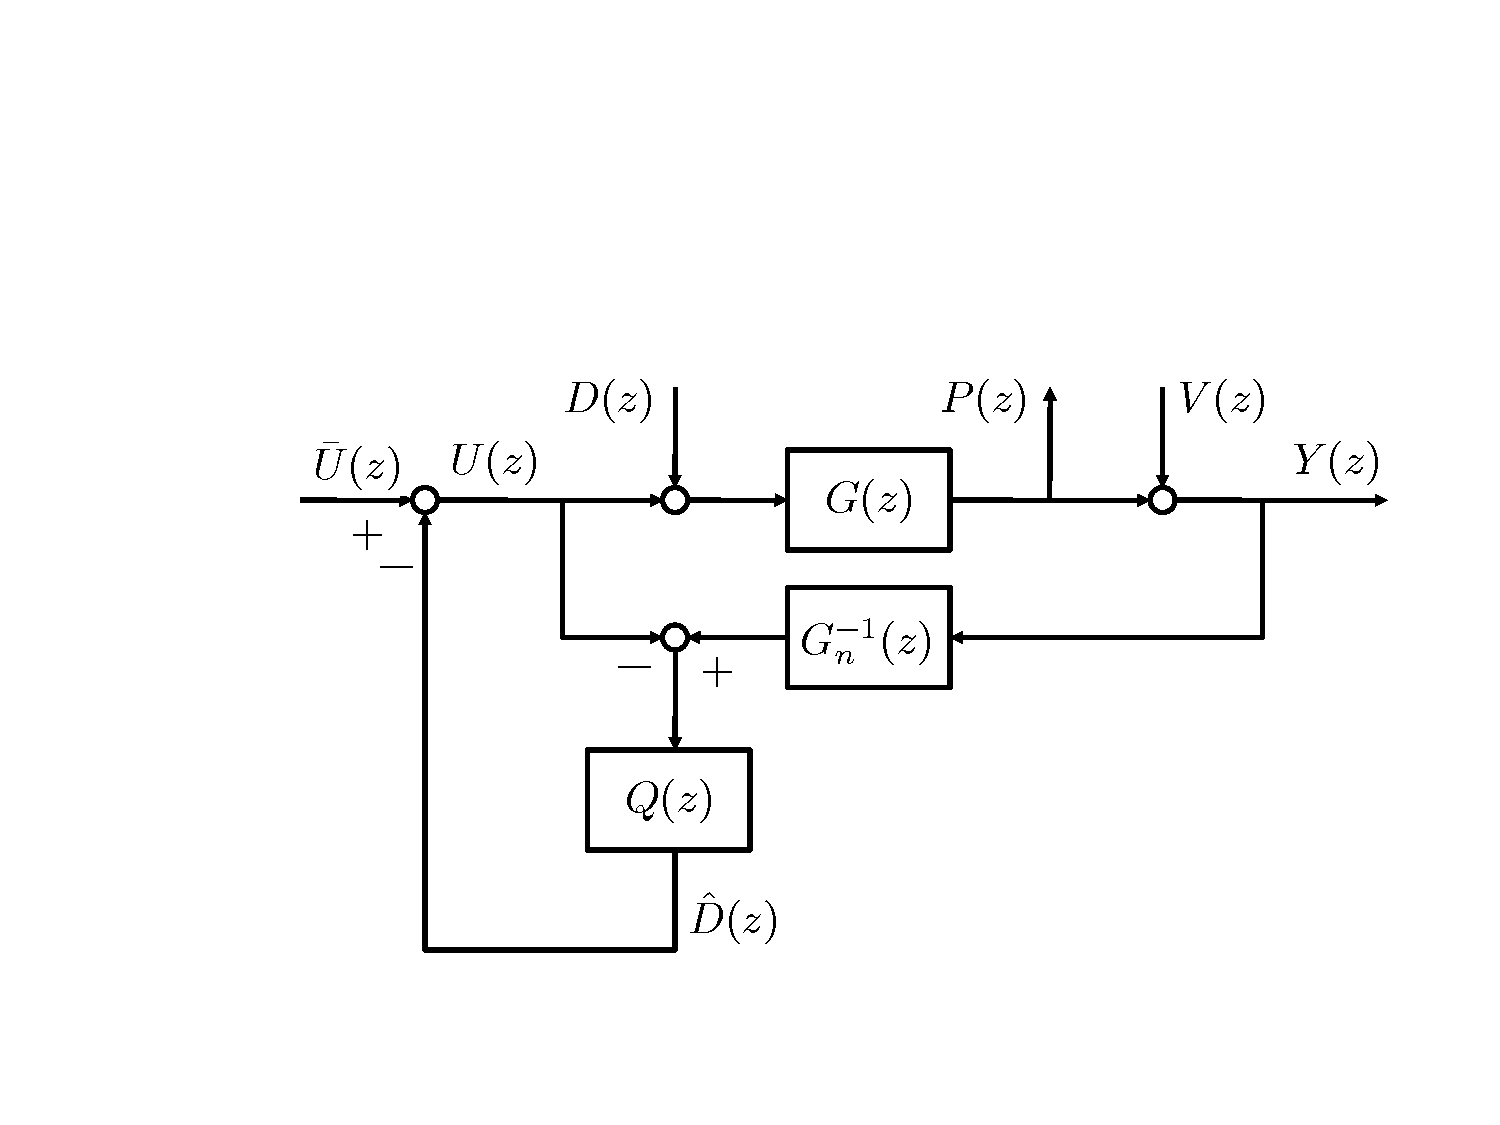
\includegraphics[width=0.5\textwidth]{Disturbance_Observer_DO}\\
    \end{figure}

    Concerns when choosing $Q(z)$:
    \begin{enumerate}
    \item[4.] \textbf{Realizability:}
    Choose $Q(z)$ so that $\hat{D}(z) = Q(z) [ G_n^{-1}(z) Y(z) - U(z)]$ is realizable
    \pause
    \newline

    $\Rightarrow$ Choose $Q(z)$ realizable so that $\displaystyle\frac{Q(z)}{G_n(z)}$ is also realizable
    \pause
    \newline

    This is a constraint on the relative degree of $Q(z)$

    \end{enumerate}
\end{frame} 
\section{Adding a disturbance observer to an existing feedback controller}
\begin{frame}
    \frametitle{Outline}
    \tableofcontents[currentsection]
\end{frame}

\begin{frame}
    \frametitle{Adding a disturbance observer to an existing controller}

    Suppose we have designed a controller $C(z)$ for the interconnection
    \begin{figure}
        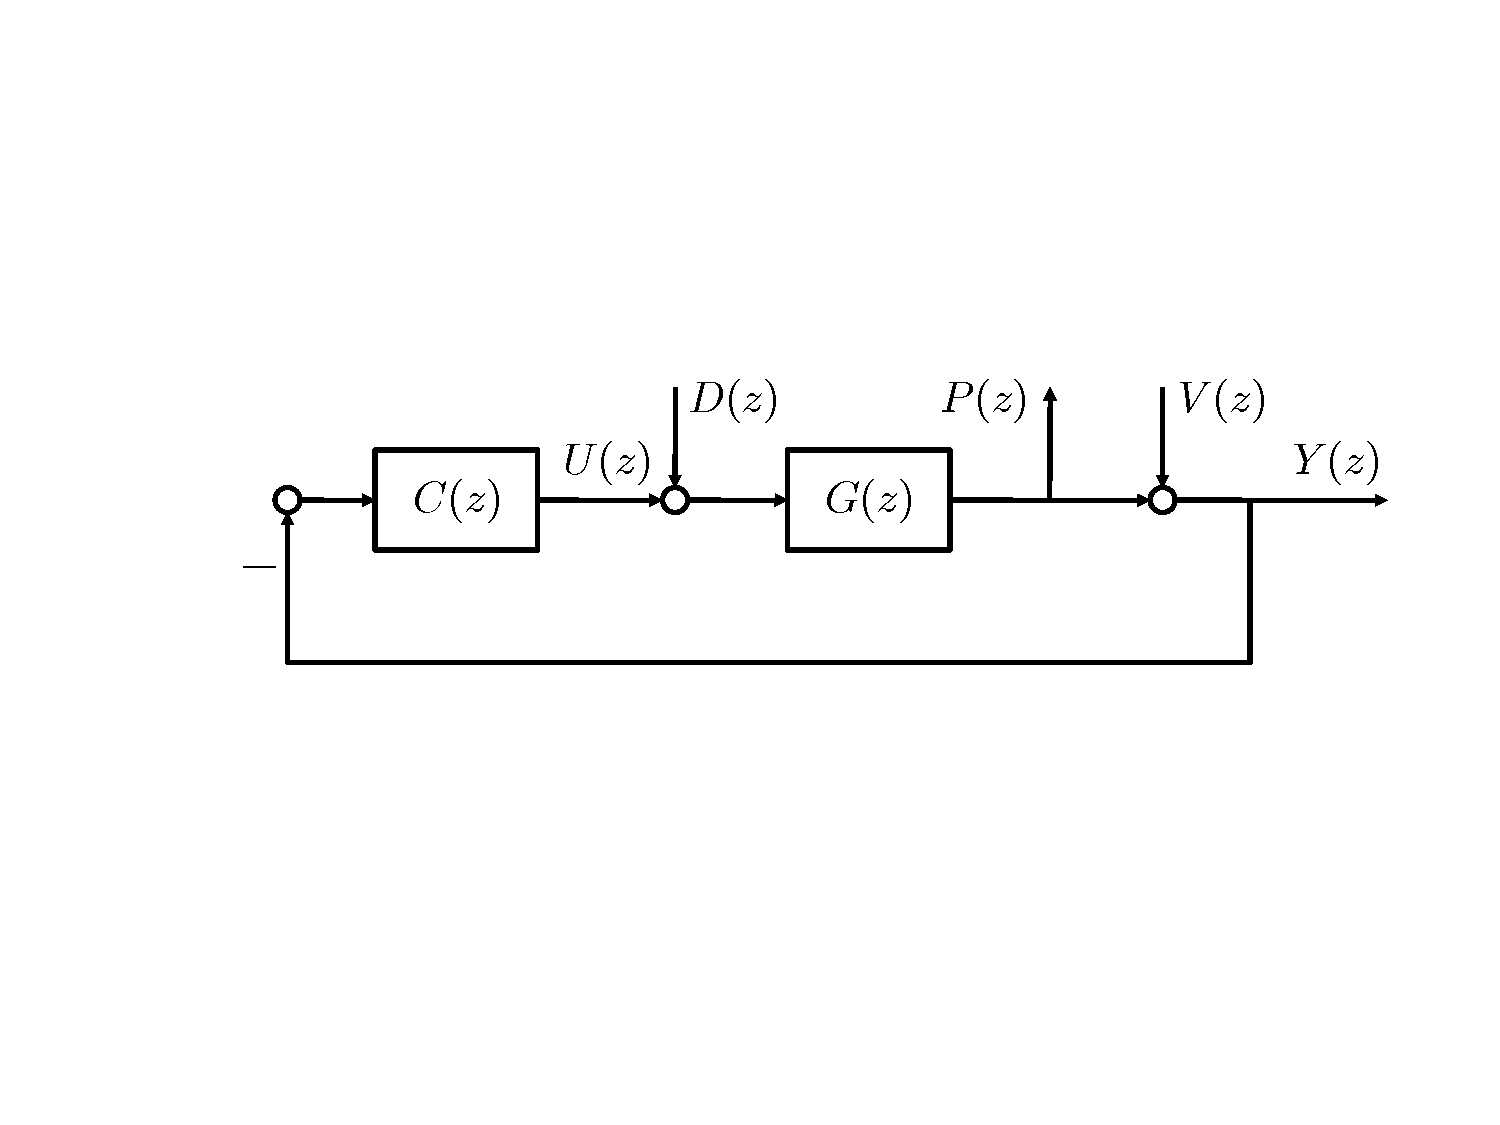
\includegraphics[width=0.5\textwidth]{Disturbance_Observer_multi1}
    \end{figure}
    and we would like to add a disturbance observer:
    \begin{figure}
        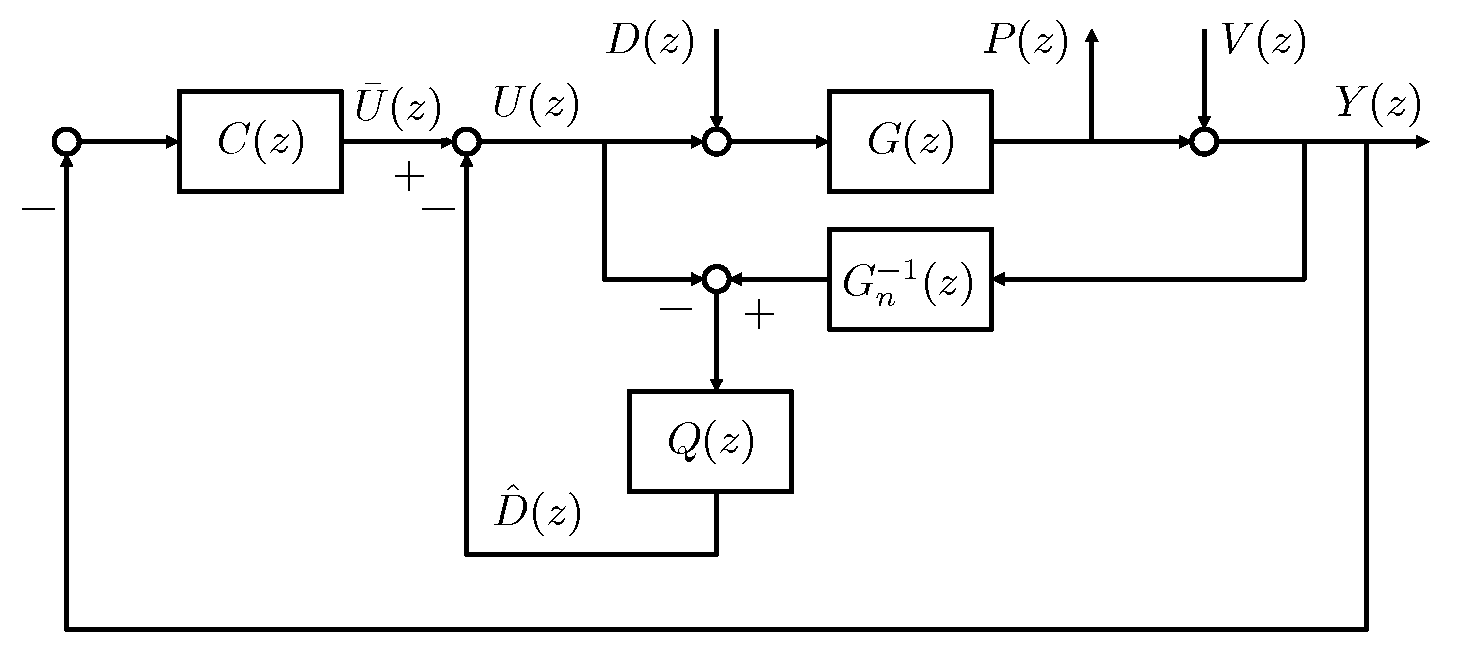
\includegraphics[width=0.5\textwidth]{Disturbance_Observer_multi2}
    \end{figure}
    \pause
    How does this affect the stability of the closed-loop system?

\end{frame}

\begin{frame}
    \frametitle{Adding a disturbance observer to an existing controller}

    \begin{figure}
        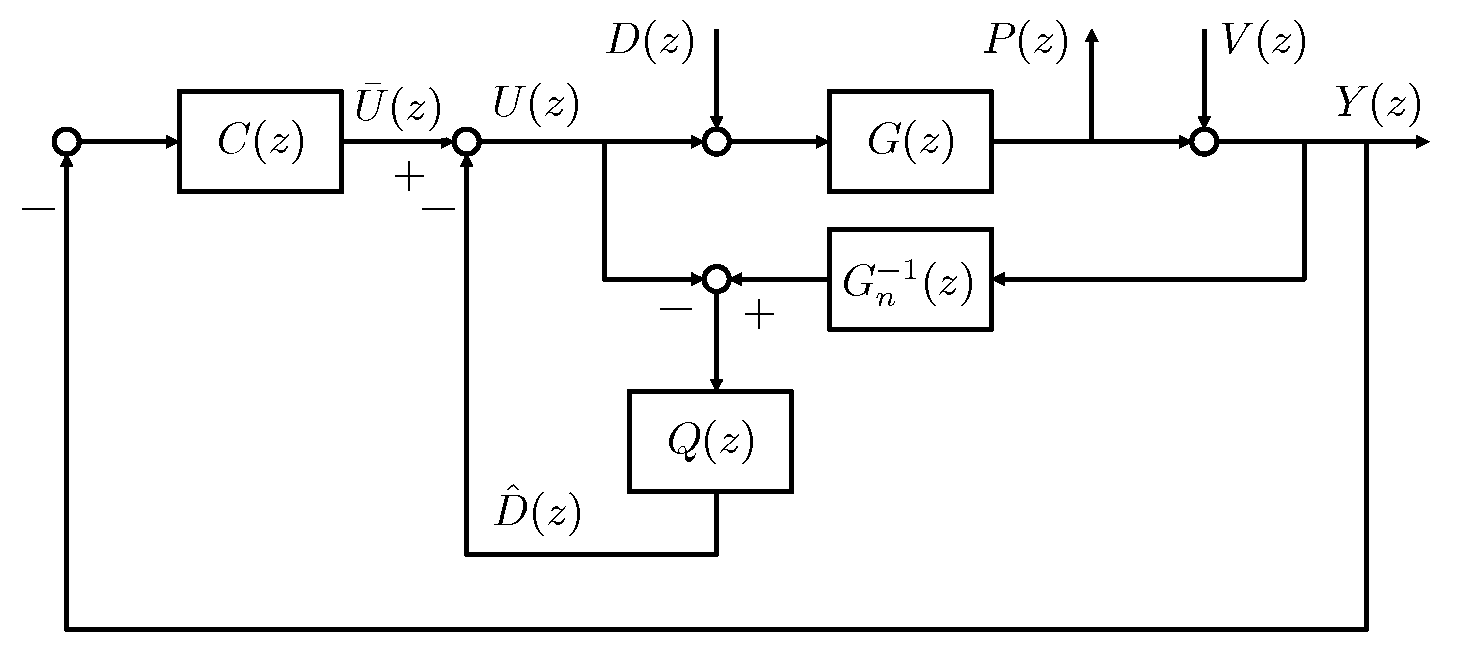
\includegraphics[width=0.4\textwidth]{Disturbance_Observer_multi2}
    \end{figure}
    Since we are only interested in stability, we set the exogenous inputs to zero. Also, we let $G(z) = G_n(z) ( 1 + \Delta(z))$.
    \pause
    \begin{figure}
        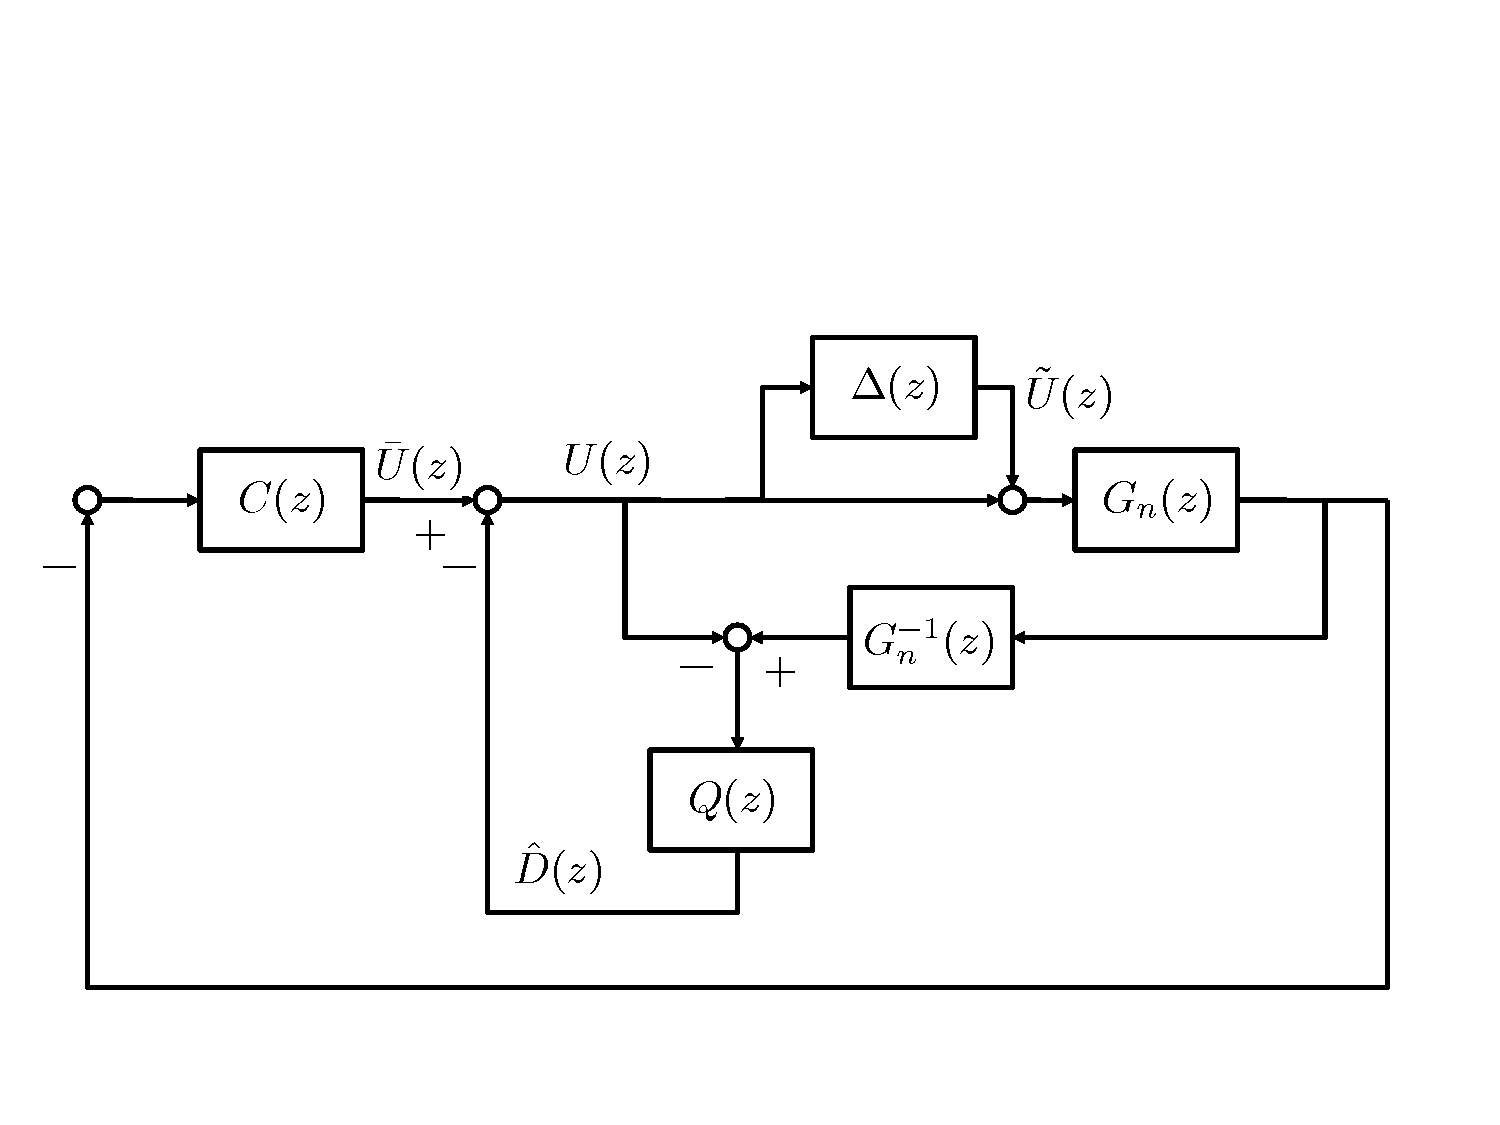
\includegraphics[width=0.5\textwidth]{Disturbance_Observer_multi3}
    \end{figure}
    \pause

    To use the small-gain theorem, we must simplify this to a feedback interconnection of $\Delta(z)$ and another system.

\end{frame}

\begin{frame}
    \frametitle{Simplifying the closed-loop representation}

    Removing $\Delta(z)$ from the interconnection, we have
    \begin{figure}
        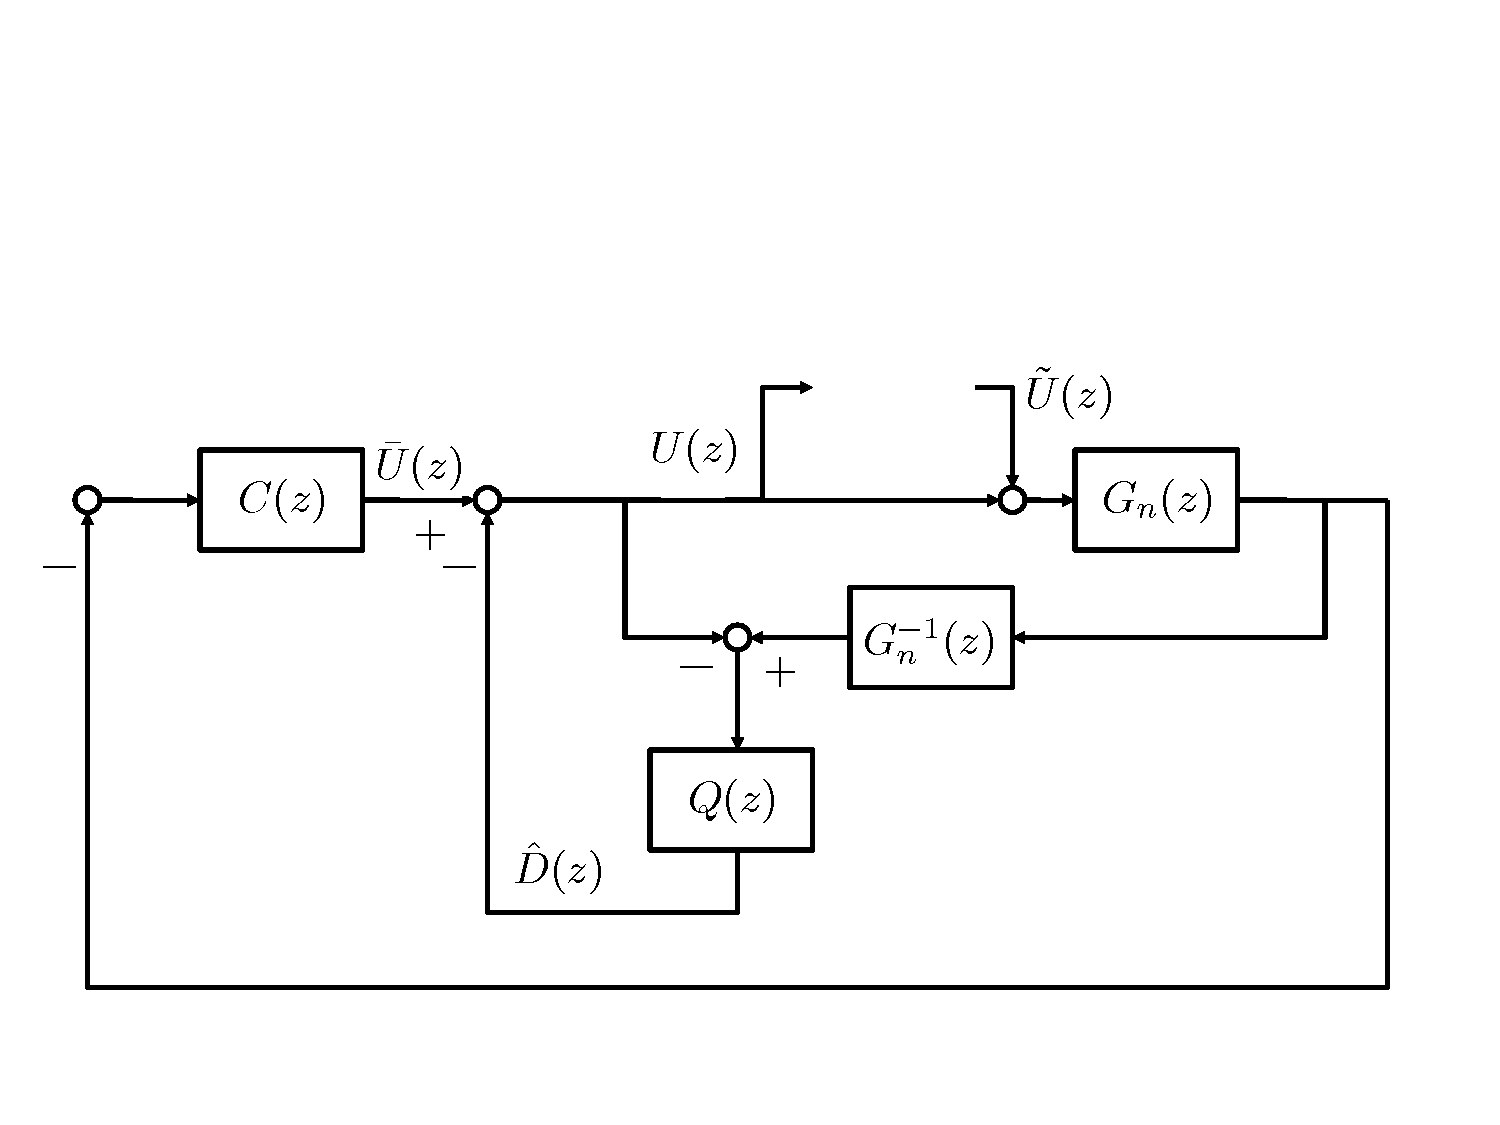
\includegraphics[width=0.5\textwidth]{Disturbance_Observer_multi4}
    \end{figure}
    \pause
    Omitting dependency on $z$, we have
    \begin{gather*}
        \hat{D} = Q \left[ \frac{G_n}{G_n}(\tilde{U} + U) - U \right]
            \quad \Rightarrow \quad \hat{D} = Q \tilde{U} \\
        U = -CG_n (\tilde{U} + U) - \hat{D}
            \quad \Rightarrow \quad U = -CG_n(\tilde{U} + U) - Q \tilde{U} \\
        \Rightarrow \quad (1 + CG_n) U = -(CG_n + Q) \tilde{U}
    \end{gather*}

\end{frame}

\begin{frame}
    \frametitle{Closed-loop stability}

    We now have the simplified closed-loop system representation
    \begin{figure}
        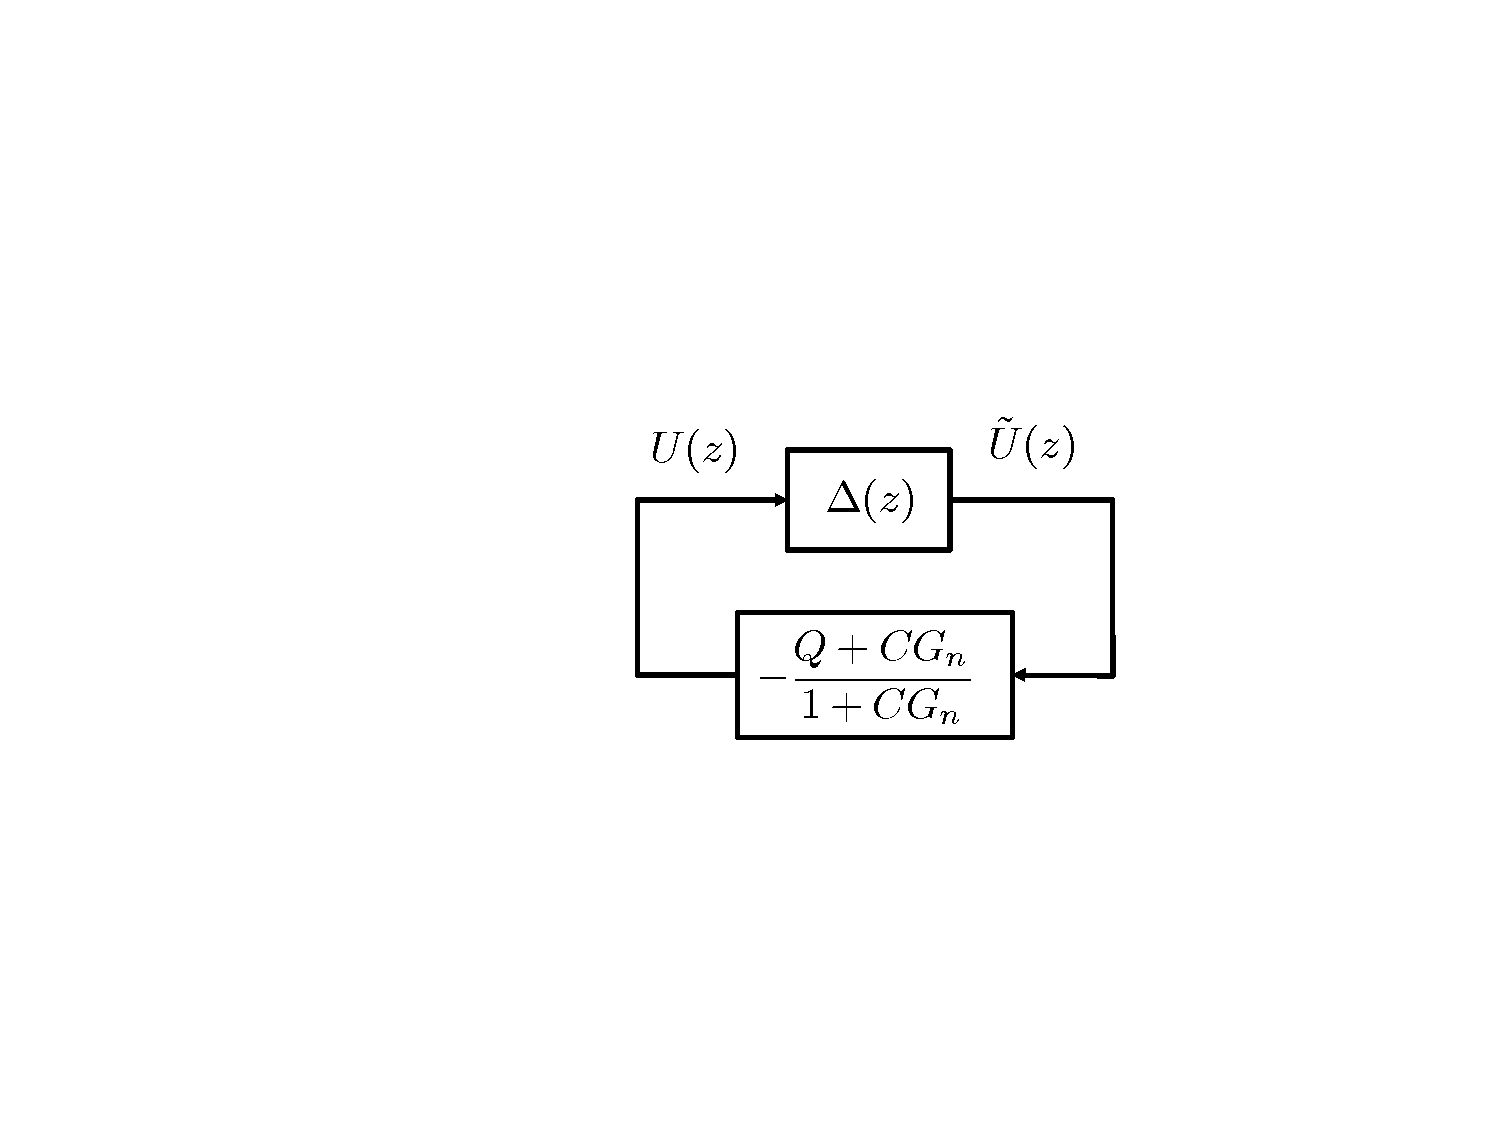
\includegraphics[width=0.3\textwidth]{Disturbance_Observer_multi5}
    \end{figure}
    \pause
    Using the small-gain theorem, we can therefore guarantee closed-loop stability if:
    \begin{enumerate}
    \item
    $G_n(z)$ is minimum phase
    \pause

    \item
    The following feedback interconnection is stable
    \begin{figure}
        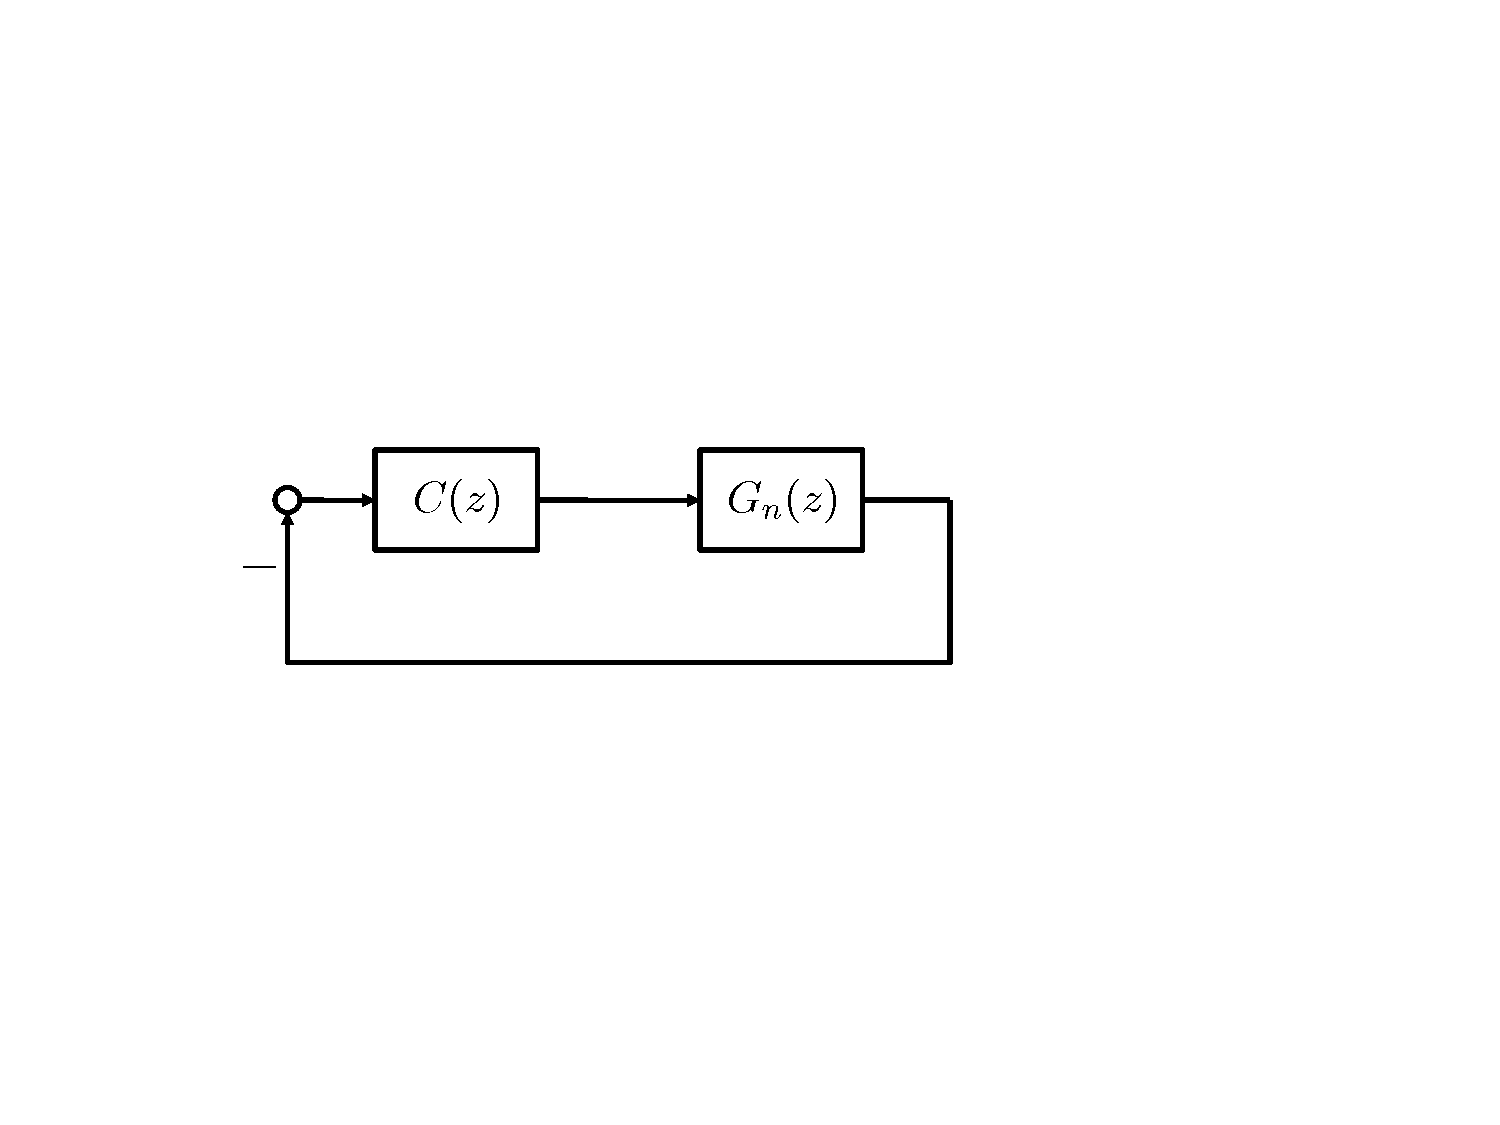
\includegraphics[width=0.3\textwidth]{Disturbance_Observer_multi6}
    \end{figure}
    \pause
    (i.e.\ the \underline{nominal} closed-loop system \underline{without} the disturbance observer is stable)
    \end{enumerate}

\end{frame}

\begin{frame}
    \frametitle{Closed-loop stability}

    We now have the simplified closed-loop system representation
    \begin{figure}
        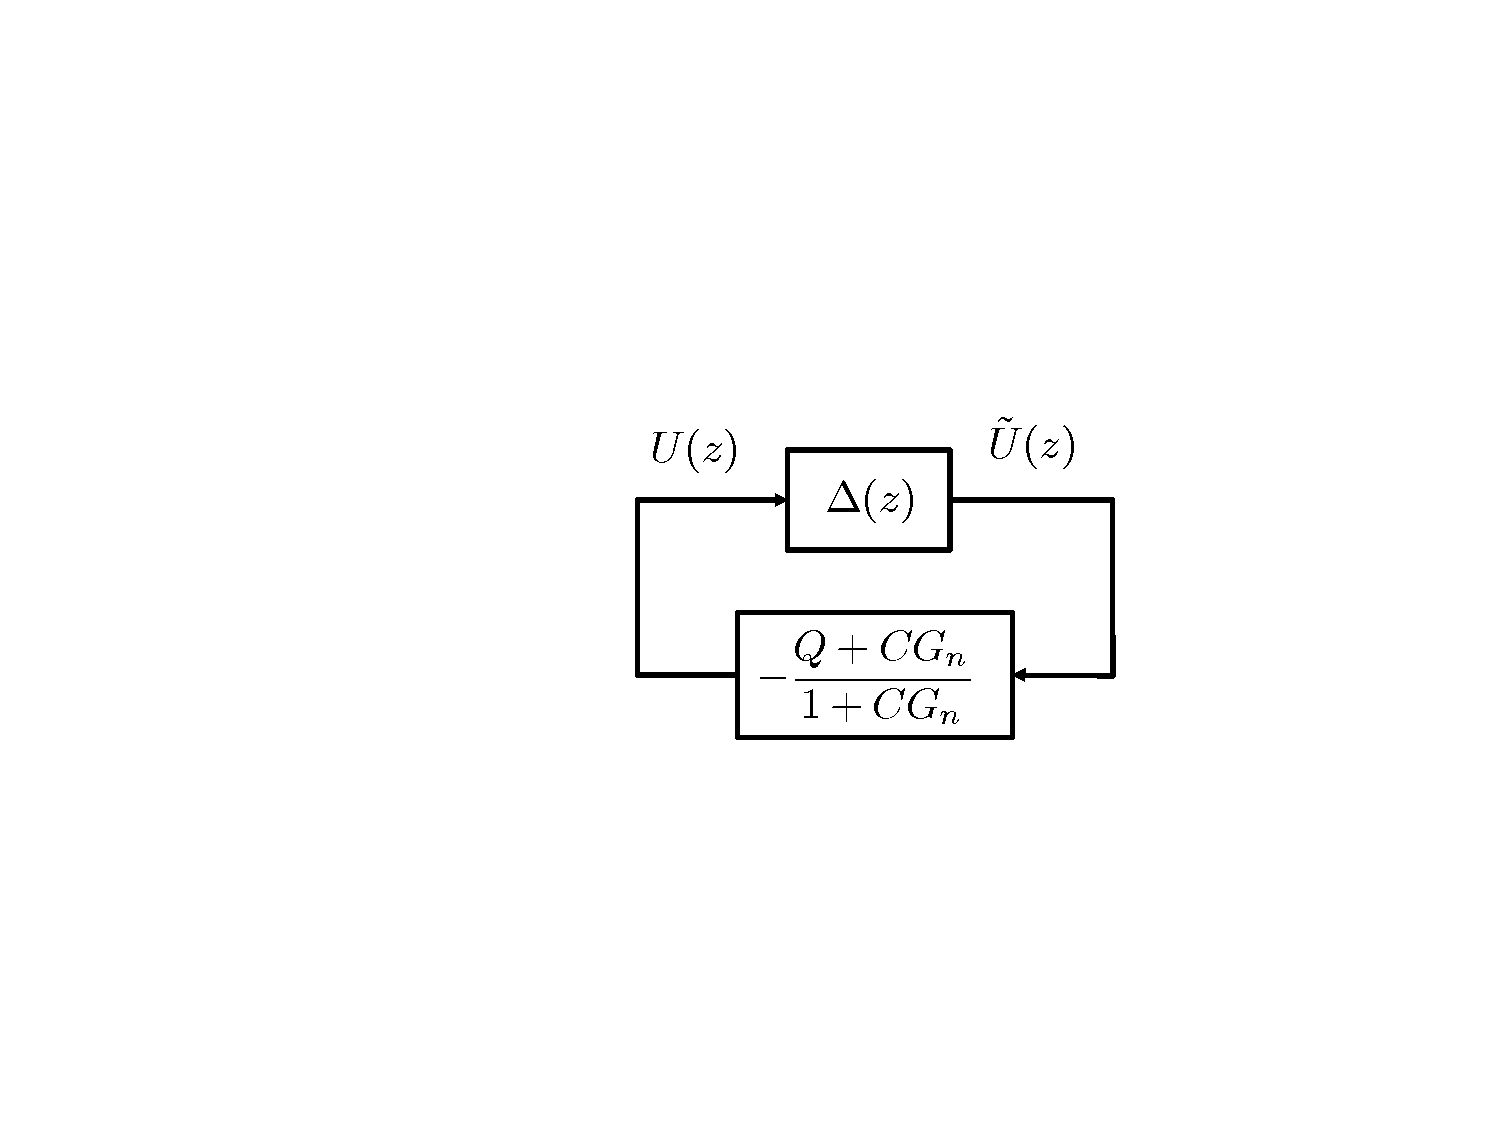
\includegraphics[width=0.3\textwidth]{Disturbance_Observer_multi5}
    \end{figure}
    Using the small-gain theorem, we can therefore guarantee closed-loop stability if:
    \begin{enumerate}
    \item[3.]
    $\displaystyle\left| \frac{Q(\ejw) + C(\ejw) G_n(\ejw)}{1 + C(\ejw) G_n(\ejw) } \right| < \frac{1}{|\Delta(\ejw)|}, \quad \forall \omega \in [0,\pi]$
    \pause
    \newline

    In order to meet this condition, it must be true that $Q(\ejw) \not\approx 1$ whenever $\omega \in [0,\pi]$ is such that $|\Delta(\ejw)| \geq 1$.

    \end{enumerate}

\end{frame}





\end{document} 